\subsection{Vorbereitung}
Zur Vorbereitung sollen die Dopplerwinkel $\alpha$ zu verschiedenen Prismenwinkeln
$\theta$
mit Formel \eqref{eqn:alpha} berechnet werden. Die Ergebnisse finden sich in
Tabelle \ref{tab:alpha} wieder.
\begin{table}
  \centering
  \begin{tabular}{c|c}
    \toprule
    $\theta\,/\dgr$ & $\alpha\,/\dgr$ \\
    \midrule
    $ 0$ & $90.00$ \\
    $15$ & $80.06$ \\
    $30$ & $70.54$ \\
    $60$ & $54.73$ \\
    \bottomrule
  \end{tabular}
  \caption{Doppler-Winkel für verschiedene Prismenwinkel.}
  \label{tab:alpha}
\end{table}
\subsection{Bestimmung der Fließgeschwindigkeit}
\begin{wrapfigure}{r}{5cm}
  \centering
  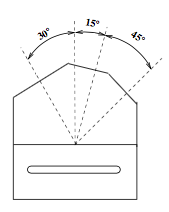
\includegraphics[width=3.5cm]{bilder/winkel.png}
  \caption{Doppler-Prisma mit den Winkeln $15\dgr$, $30\dgr$ und $60\dgr$ \cite{us3}.}
  \label{fig:prisma}
\end{wrapfigure}
Die Fließgeschwindigkeiten werden in drei Rohren mit den Innendurchmessern von
$d_1 = 7\mm$, $d_2 = 10\mm$ und $d_3=16\mm$ mit dem Impuls-Echo-Verfahren bestimmt.
Dabei werden die Frequenzverschiebungen zu jeweils fünf verschiedenen
Fließgeschwindigkeiten bestimmt, welche über die Leistung der Pumpe reguliert werden.
Um die Doppler-Winkel $\theta$ einzuhalten wird der Doppler-Prisma aus Abb. \ref{fig:prisma} verwendet.
Die entsprechenden Frequenzverschiebungen zu den verschiedenen Pumpleistungen in den verschiedenen Rohren sind in \ref{tab:helga} zu finden.
Die Geschwindigkeiten werden mit
\begin{equation}
  v = \frac{\Delta \nu c}{2 \nu_0 \cos{\alpha}} \label{eqn:v}
\end{equation}
ausgerechnet. Für die Geschwindigkeit im Prisma gilt $c_\su{P}= 2700\vel$, in der
Dopplerflüssigkeit gilt $c_\su{Fl}=1800\vel$. Die benötigten Winkel $\alpha$ sind in Tabelle \ref{tab:alpha} aufgelistet.
\begin{table}[H]
  \centering
  \begin{tabular}{|c|c|ccc|}
    \toprule
    \mc{1}{|c|}{Rohrdurchmesser}&\mc{1}{c|}{Prismenwinkel}&\mc{1}{c}{Frequenzverschiebung}&
    \mc{1}{c}{Geschwindigkeit}&\mc{1}{c|}{Pumpleistung} \\
    $\mm$&$\su{\theta}$&$\Hz$&$\vel$&\% \\
    \midrule
    \mr{15}{*}{16}&\mr{5}{*}{15}&   73 & 0.19 & 35.2 \\
                  &             &   85 & 0.22 & 45.2 \\
                  &             &   98 & 0.26 & 50.0 \\
                  &             &  122 & 0.32 & 55.2 \\
                  &             &  171 & 0.44 & 70.0 \\ \cline{2-5}
                  &\mr{5}{*}{30}&   85 & 0.11 & 35.2 \\
                  &             &  122 & 0.16 & 45.2 \\
                  &             &  134 & 0.18 & 50.0 \\
                  &             &  171 & 0.23 & 55.2 \\
                  &             &  256 & 0.35 & 70.0 \\ \cline{2-5}
                  &\mr{5}{*}{60}&  143 & 0.11 & 35.2 \\
                  &             &  195 & 0.15 & 45.2 \\
                  &             &  232 & 0.18 & 50.0 \\
                  &             &  281 & 0.22 & 55.2 \\
                  &             &  452 & 0.35 & 70.0 \\ \cline{1-5}
    \mr{15}{*}{10}&\mr{5}{*}{15}&  110 & 0.29 & 35.2 \\
                  &             &  159 & 0.41 & 45.2 \\
                  &             &  208 & 0.54 & 50.0 \\
                  &             &  220 & 0.57 & 55.2 \\
                  &             &  330 & 0.86 & 70.0 \\ \cline{2-5}
                  &\mr{5}{*}{30}&  171 & 0.23 & 35.2 \\
                  &             &  244 & 0.33 & 45.2 \\
                  &             &  305 & 0.41 & 50.0 \\
                  &             &  366 & 0.49 & 55.2 \\
                  &             &  598 & 0.81 & 70.0 \\ \cline{2-5}
                  &\mr{5}{*}{60}&  269 & 0.21 & 35.2 \\
                  &             &  464 & 0.36 & 45.2 \\
                  &             &  574 & 0.45 & 50.0 \\
                  &             &  720 & 0.56 & 55.2 \\
                  &             & 1062 & 0.83 & 70.0 \\ \hline
    \mr{15}{*}{6} &\mr{5}{*}{15}&  171 & 0.44 & 35.2 \\
                  &             &  293 & 0.76 & 45.2 \\
                  &             &  330 & 0.86 & 50.0 \\
                  &             &  415 & 1.08 & 55.2 \\
                  &             &  647 & 1.68 & 70.0 \\ \cline{2-5}
                  &\mr{5}{*}{30}&  317 & 0.43 & 35.2 \\
                  &             &  513 & 0.69 & 45.2 \\
                  &             &  676 & 0.91 & 50.0 \\
                  &             &  891 & 1.20 & 55.2 \\
                  &             & 1355 & 1.83 & 70.0 \\ \cline{2-5}
                  &\mr{5}{*}{60}&  476 & 0.37 & 35.2 \\
                  &             &  793 & 0.62 & 45.2 \\
                  &             &  964 & 0.75 & 50.0 \\
                  &             & 1233 & 0.96 & 55.2 \\
                  &             & 1941 & 1.51 & 70.0 \\
   \bottomrule
  \end{tabular}
  \caption{Frequenzverschiebungen/ Geschwindigkeiten zu den verschiedenen Einstrahlwinkel in den
  drei Rohren.}
  \label{tab:helga}
\end{table}
\newpage
\noindent In Tabelle \ref{tab:mittelwerte} sind die gemittelten Geschwindigkeiten
der drei verwendeten Rohrdurchmesser für die jeweiligen Pumpleistungen
zu finden.
\begin{table}[H]
\centering
\begin{tabular}{ccc}
  \toprule
  Rohrdurchmesser$/\mm$ & Pumpleistung $/\,\%$ & Geschwindigkeit$/\vel$ \\
  \midrule
      \mr{5}{*}{7}        &   35.2    & 0.42 \pm \, 0.03      \\
                          &   45.2    & 0.69 \pm \, 0.06      \\
                          &   50.0    & 0.84 \pm \, 0.07      \\
                          &   55.2    & 1.08 \pm \, 0.10      \\
                          &   70.0    & 1.68 \pm \, 0.13      \\ \midrule
     \mr{5}{*}{10}        &   35.2    & 0.24 \pm \, 0.03      \\
                          &   45.2    & 0.37 \pm \, 0.03      \\
                          &   50.0    & 0.47 \pm \, 0.05      \\
                          &   55.2    & 0.54 \pm \, 0.04      \\
                          &   70.0    & 0.83 \pm \, 0.02      \\ \midrule
     \mr{5}{*}{16}        &   35.2    & 0.14 \pm \, 0.04      \\
                          &   45.2    & 0.18 \pm \, 0.03      \\
                          &   50.0    & 0.21 \pm \, 0.04      \\
                          &   55.2    & 0.26 \pm \, 0.04      \\
                          &   70.0    & 0.38 \pm \, 0.05      \\
  \bottomrule
\end{tabular}
\caption{Die gemittelten Geschwindigkeiten für die verschiedenen Rohrdurchmesser.}
\label{tab:mittelwerte}
\end{table}
Anschließend werden für die drei Rohre die drei Abbildungen \ref{fig:dünn}, \ref{fig:mittel}
und \ref{fig:dick} erstellt. In jeder Abbildung befinden sich jeweils drei Graphen für die drei verwendeten Einstrahlwinkel $\theta$. Dabei wird
$\frac{\Delta \nu}{\cos{\alpha}}$ gegen die Strömungsgeschinwigkeit aufgetragen.
\begin{figure}[H]
  \centering
  \includegraphics[width=0.8\textwidth]{bilder/winkelduenn.pdf}
  \caption{Dopplerwinkel in Abhängigkeit der Strömungsgeschwindigkeit beim dünnen
  Rohr.}
  \label{fig:dünn}
\end{figure}
\begin{figure}[H]
  \centering
  \includegraphics[width=0.8\textwidth]{bilder/winkelmittel.pdf}
  \caption{Dopplerwinkel in Abhängigkeit der Strömungsgeschwindigkeit beim mittleren
  Rohr.}
  \label{fig:mittel}
\end{figure}
\begin{figure}[H]
  \centering
  \includegraphics[width=0.8\textwidth]{bilder/winkeldick.pdf}
  \caption{Dopplerwinkel in Abhängigkeit der Strömungsgeschwindigkeit beim dicken
  Rohr.}
  \label{fig:dick}
\end{figure}
\newpage
\subsection{Bestimmung des Geschwindigkeitsprofils}
Um das Strömungsprofil zu bestimmen wird das mittlere Rohr verwendet mit
$d_2 = 10\mm$, welches dem $\sfrac{3}{8}$ Zoll Rohr entspricht. Dabei wird
ein Einstrahlwinkel von $\theta = 15\dgr$ verwendet. In Tabelle \ref{tab:rita} befinden
sich die Werte bei $45\,\%$ Pumpleistung und in Tabelle \ref{tab:hilde} die Werte
bei $70\,\%$ Leistung. Hierbei wird zuvor die Tiefe eingestellt, da nur die Frequenzverschiebung im Rohr gemessen werden soll. Dazu wird aus der Anleitung
entnommen, dass die Vorlaufstrecke im Prisma $l=30.7\mm$ entspricht. Für diese Strecke gilt $10\mm = 4\ms$ und somit $t=12.28\ms$. Für den Startwert von $t=13.28\ms$ wird zusätzlich noch die Dicke des Rohrs von
$2.5\mm$ mit einbezogen. Deswegen beginnt
die Messung bei $t=13.0\ms$. Jedoch befindet sich erst der Wert $t=13.5\ms$ in der
Dopplerflüssigkeit. In der Dopplerflüssigkeit gilt $6\mm = 4\ms$.
\begin{table}[H]
  \centering
  \begin{tabular}{cccc}
    \toprule
    \mc{1}{c}{Laufzeit}&\mc{1}{c}{Frequenzverschiebung}&\mc{1}{c}{Streuintensität}&
    \mc{1}{c}{Geschwindigkeit} \\
    $\ms$&$\Hz$&$1000\frac{\Volt^2}{\sek}$&$\vel$ \\
    \midrule
    13.0 & 220 & 184 & 0.57 \\
    13.5 & 232 & 214 & 0.60 \\
    14.0 & 245 & 235 & 0.64 \\
    14.5 & 256 & 228 & 0.67 \\
    15.0 & 269 & 220 & 0.70 \\
    15.5 & 256 & 222 & 0.67 \\
    16.0 & 244 & 221 & 0.64 \\
    16.5 & 232 & 214 & 0.60 \\
    17.0 & 195 & 124 & 0.51 \\
    17.5 & 195 & 124 & 0.51 \\
    \bottomrule
  \end{tabular}
  \caption{Frequenzverschiebung/ Geschwindigkeiten und Streuintensität des mittleren Rohrs bei
  $45\,\%$ Pumpleistung.}
  \label{tab:rita}
\end{table}

\begin{table}[H]
  \centering
  \begin{tabular}{cccc}
    \toprule
    \mc{1}{c}{Laufzeit}&\mc{1}{c}{Frequenzverschiebung}&\mc{1}{c}{Streuintensität}&
    \mc{1}{c}{Geschwindigkeit} \\
    $\ms$&$\Hz$&$1000\frac{\Volt^2}{\sek}$&$\vel$ \\
    \midrule
    13.0 & 415 & 307 & 1.08 \\ % 0.57
    13.5 & 427 & 374 & 1.11 \\ % 0.60
    14.0 & 476 & 388 & 1.24 \\ % 0.64
    14.5 & 500 & 406 & 1.30 \\ % 0.67
    15.0 & 513 & 415 & 1.34 \\ % 0.70
    15.5 & 500 & 410 & 1.30 \\ % 0.67
    16.0 & 476 & 401 & 1.24 \\ % 0.64
    16.5 & 427 & 437 & 1.11 \\ % 0.60
    17.0 & 341 & 161 & 0.89 \\ % 0.51
    17.5 & 341 & 161 & 0.89 \\ % 0.51
    \bottomrule
  \end{tabular}
  \caption{Frequenzverschiebung/ Geschwindigkeiten und Streuintensität des mittleren Rohrs bei
  $70\,\%$ Pumpleistung.}
  \label{tab:hilde}
\end{table}
In Graph \ref{fig:profil} befinden sich die Geschwindigkeitsprofile bei jeweils
$45\,\%$ und $70\,\%$ Pumpleistung. Dabei wird die Strömungsgeschwindigkeit gegen
die Eindringtiefe in $\ms$ dargestellt.
\begin{figure}
  \centering
  \includegraphics[width=0.8\textwidth]{bilder/profilV.pdf}
  \caption{Geschwindigkeitsprofile für $45\,\%$ und $70\,\%$ Pumpleistung.}
  \label{fig:profil}
\end{figure}
In Abb. \ref{fig:streu} sind die Graphen zu den Streuintensitäten zu beiden
Pumpleistungen wiederzufinden. Dabei wird die Streuintensität gegen die Eindringtiefe
aufgetragen.
\begin{figure}
  \centering
  \includegraphics[width=0.8\textwidth]{bilder/streuintensitaet.pdf}
  \caption{Streuintensitäten für $45\,\%$ und $70\,\%$ Pumpleistung.}
  \label{fig:streu}
\end{figure}
